\chapter{Circuitos secuenciales}

Aunque hemos comentado con profusión los circuitos combinacionales, lo que realmente impera en la práctica son los circuitos secuenciales. Mientras que hemos visto que en los circuitos combinacionales la salida depende exclusivamente de los valores de las entradas en el momento actual, en los circuitos secuenciales se tienen los valores de las entradas en el pasado. Por ejemplo, si tenemos un ventilador con diferentes velocidades y queremos aumentarla, tenemos que saber algo más aparte de una entrada que indique el incremento de la velocidad. Es decir, tendría que haber un estado que nos indique la velocidad actual del sistema para saber cómo incrementar la velocidad. Es aquí donde entran en juego las \emph{máquinas de estado.}

\section{Máquinas de estado.}

El funcionamiento de un sistema como el ventilador puede ser conceptualizada como un conjunto de estados interrelacionados, es decir, una \hyperlink{state-machine}{máquina de estados.} El estado de un circuito secuencial puede definirse como ``una colección de \emph{variables de estado} cuyos valores en cualquier instante contienen toda la información acerca del pasado necesaria para predecir el comportamiento del circuito en el futuro'' \textcolor{red}{CITAR LIBRO DE HERERT HELLERMAN DIGITAL COMPUTER SYSTEM PRINCIPLES DE 1967}. No obstante, son necesarias más cosas aparte de variables de estado, por ejemplo, se necesita saber hacia qué estado. Este no solo dependerá del valor de las entradas del sistema, sino del estado en el que se encuentre en ese momento. En el ejemplo del ventilador, si activamos la señal de incremento de la velocidad y nos encontramos en el estado \emph{VELOCIDAD\_MEDIA}, el circuito se moverá al estado \emph{VELOCIDAD\_ALTA}. Por el contrario, para la misma entrada, si el circuito se encontrara en el estado \emph{VELOCIDAD\_BAJA}, éste cambiaría a \emph{VELOCIDAD\_MEDIA}. Como el númerod de estados de un sistema no es infinito, las máquinas de estado (y los circuitos secuenciales en general) se suelen conocer también por el nombre de \emph{máquinas de estados finitos.}

En los circuitos secuenciales cobra gran importancia el \emph{reloj}, ya que los cambios entre estados deben llevarse a cabo de manera sincronizada. En la mayoría de sistemas, el cambio de estado se lleva a cabo en los \hyperlink{edge}{\emph{flancos}} del reloj, o \hyperlink{active_edge}{\emph{flancos activos/gatillo}}, ya sea de subida o de bajada (aunque es más frecuente en el de subida). Una señal de reloj es \hyperlink{active_high}{\emph{activa en alto}} si los cambios de estado se producen en el flanco de subida, o \hyperlink{active_low}{\emph{activa en bajo}} si los cambios se llevan a cabo en el flanco de bajada. Este tipo de relojes debe estár activo, funcionando a una frecuencia dada y regular, mientras el circuito esté activo. Esta señal de reloj con frecuencia es generada por un oscilador de cristal de cuarzo, cuya frecuencia varía dependiendo del circuito en el que se integre.

Otro elemento a tener en cuenta en los circuitos secuenciales es el de \hyperlink{flip-flop}{biestable}. Estos son elementos con memoria, que permiten mantener el valor de las variables de estado, entre otras cosas. Un biestable se puede implementar por medio de un \hyperlink{feedback_sequential_circuit}{\emph{circuito secuencial retroalimentado}}, en el cual un bucle de retroalimentación se incluye en el circuito secuencial para añadir memoria al sistema. Hay multitud de tipos de biestables:

\begin{itemize}
    \item \emph{Biestable SR.}
    \item \emph{Biestable JK.}
    \item \emph{Biestable D.}
    \item \emph{Biestable T.}
\end{itemize}

\subsection{Estructura de las máquinas de estado}

La mayoría de máquinas de estado actuales son \hyperlink{clocked_synchronous_state_machine}{\emph{máquinas de estado sincronizadas por reloj}} que usan biestables D disparados por flanco. Son sincronizados por reloj porque todos los biestables están conectados a la misma señal de reloj, cambiando al mismo tiempo su estado en respuesta a los flancos del reloj. Las Figuras \ref{fig:mef-mealy} y \ref{fig:mef-moore} muestran la estructura general de una máquina de estados finitos de Mealy y de Moore, respectivamente. Ambas tienen en común una \emph{memoria de estado}, que está constituida por un conjunto de $n$ biestables que almacenan el estado del circuito. A estos biestables se les conecta una \emph{señal de reloj} común, the tal manera que el estado sólo cambia en los \emph{tics} del reloj. El \emph{tic} (se podría definir como el instante en el que cambia el estado) depende del tipo de biestable usado. Por ejemplo, para los biestables que se activan en el flanco de subida, el tic es el flanco de subida del reloj. El estado siguiente de la máquina de estados viene determinado por la \emph{lógica del estado siguiente} que es función del estado actual y las entradas. En cambio, la \emph{lógica de salida} depende del tipo de circuito del que se trate. En las máquinas de estados finitos de Mealy, la lógica de salida viene determinada por las entradas y el estado actual.

\begin{figure}[h]
    \centering
    \includegraphics[width=\textwidth]{figs/mef-mealy.drawio.png}
    \caption[short]{Máquina de estados finitos de Mealy.}
    \label{fig:mef-mealy}
\end{figure}

En cambio, en una máquina de estados finitos de Moore, la lógica de salida viene determinada exclusivamente del estado actual.

\begin{figure}[h]
    \centering
    \includegraphics[width=\textwidth]{figs/mef-moore.drawio.png}
    \caption[short]{Máquina de estados finitos de Moore.}
    \label{fig:mef-moore}
\end{figure}

Como se puede observar en los diagramas, la única diferencia entre ambos tipos de modelos radica en cómo se generan las salidas. 

En el diseño de circuitos de gran velocidad es necesario que las salidas estén disponibles lo antes posible. Por ello, en ocasiones se codifican las variables de estado para que sirvan de salida también. Este tipo de diseño se denomina \hyperlink{output-coded_state_assignment}{\emph{asignación de estados codificada en salidas}}. En este caso la salida del circuito consiste en \verb|wires|. Otra manera de abordar el diseño de una máquina de estados es haciendo que la salida durante un periodo de reloj dependa de la salida en el periodo de reloj anterior. Esto se denomina \hyperlink{pipelined_outputs}{\emph{salida por etapas}} y se consigue uniendo otra etapa de memoria, llamada \emph{memoria de salida por etapas}, a las salidas del circuito.

\subsection{Temporización de las máquinas de estados}

\textcolor{red}{POR HACER}

\section{Diseño de máquinas de estado con tablas de estado}

\textcolor{red}{POR HACER (pag. 455)}

\section{Diseño de máquinas de estado con diagramas de estado}

\textcolor{red}{POR HACER (pag. 472)}

\section{Diseño de máquinas de estado con Verilog}

Para explicar el diseño de máquinas de estados vamos a partir de las siguientes especificaciones:

Diseña una máquina de estados síncrona con reloj con dos entradas, A y B, y una salida Z que es 1 si:

\begin{itemize}
    \item A tiene el mismo valor que en los dos tics de reloj previos.
    \item B vale uno tras la última vez que la primera condición fue cierta.
\end{itemize}

Si las condiciones no se cumplen, Z vale 0.

Para visualizar mejor estas condiciones, lo mejor es comenzar describiendo una tabla de estados y salidas. La Tabla \ref{tab:tabla-salidas-estados} muestra el resultado sobre el cual vamos a trabajar para escribir el código en Verilog.

\begin{table}
    \centering
    \begin{tblr}{
      row{2} = {c},
      row{3} = {c},
      row{4} = {c},
      row{5} = {c},
      row{6} = {c},
      row{7} = {c},
      cell{1}{2} = {c=4}{c},
      cell{8}{2} = {c=5}{c},
      hline{1,9} = {-}{},
      hline{2} = {2-5}{},
      hline{8} = {2-6}{},
    }
                        & \textbf{\textit{AB}} &                      &                      &                      &                     \\
    \textbf{\textit{S}} & \textbf{\textit{00}} & \textbf{\textit{01}} & \textbf{\textit{11}} & \textbf{\textit{10}} & \textbf{\textit{Z}} \\
    INIT                & A0                   & A0                   & A1                   & A1                   & 0                   \\
    A0                  & OK0                  & OK0                  & A1                   & A1                   & 0                   \\
    A1                  & A0                   & A0                   & OK1                  & OK1                  & 0                   \\
    OK0                 & OK0                  & OK0                  & OK1                  & A1                   & 1                   \\
    OK1                 & A0                   & OK0                  & OK1                  & OK1                  & 1                   \\
                        & S*                   &                      &                      &                      &                     
    \end{tblr}

    \caption{Tabla de salidas y estados}
    \label{tab:tabla-salidas-estados}
    \end{table}

El correspondiente módulo en Verilog se compondrá de cinco secciones:

\begin{enumerate}
    \item La declaración de las entradas, salidas y variables internas al módulo.
    \item Sentencias \verb|parameter| para asignar las variables de estado a su nombre.
    \item Un primer bloque \verb|always| para crear la memoria de estado.
    \item Un segundo bloque \verb|always| para definir el comportamiento del estado siguiente.
    \item Un tercer bloque \verb|always| para definir la lógica de salida.
\end{enumerate}

El código en Verilog resultante se muestra en el Listing \ref{lst:maquina-estado-verilog}.

\begin{mycode}[style=verilogstyle, caption={Máquina de estado en Verilog.}, label=lst:maquina-estado-verilog]
module mef (
            // reloj y reset
            input clk,
            input rst,

            // entradas
            input A,
            input B,

            // salidas (como vamos a usar codigo procedural, hay que declarar la salida como reg)
            output reg Z
           );

// senales internas
reg estado, estado_siguiente;

// asignacion de variables de estado a parametros
parameter [2:0] INIT = 3'b000;
                A0 = 3'b001;
                A1 = 3'b010;
                OK0 = 3'b011;
                OK1 = 3'b100;

// comportamiento del estado siguiente
always @(*) begin
    case(estado)
        INIT: if (A == 0) estado_siguiente = A0;
              else estado_siguiente = A1;
        A0: if (A == 0) estado_siguiente = OK0;
            else estado_siguiente = A1;
        A1: if (A == 0) estado_siguiente = A0;
            else estado_siguiente = OK1;
        OK0: if (A == 0) estado_siguiente = OK0;
             else if ((A == 0) && (B == 1)) estado_siguiente = OK1;
             else estado_siguiente = A1;
        OK1: if ((A == 0) && (B == 0))             estado_siguiente = A0;
        else if ((A == 0) && (B == 1)) estado_siguiente = OK0;
        else estado_siguiente = OK1;
        default: estado_siguiente = INIT;
    endcase
end

// logica de salida
always @(estado) begin
    case(estado)
        INIT: Z = 0;
        A0: Z = 0;
        A1: Z = 0;
        OK0: Z = 1;
        OK1: Z = 1;
        default: Z = 0;
    endcase
end

// memoria de estado
always @(posedge clk) begin
    if(rst)
        estado <= 0;
    else
        estado <= estado_siguiente;
end
endmodule
\end{mycode}

En el Listing \ref{lst:mef-verilator} se muestra el banco de pruebas en C++ \footnote{En la documentación oficial, este fichero en C++ que sirve de banco de pruebas, se denomina "wrapper" (lo cual se podría traducir como envoltorio, ya que envuelve la instancia del modelo de la UBP generada por Verilator).}. En dicho banco de pruebas vemos cómo se instancia un objeto de la UBP (\verb|Vmef *dut = new Vmef;|). Dicho objeto es generado con Verilator mediante el siguiente comando.

\begin{lcverbatim}
verilator -Wall --trace -cc <nombre-de-UBP>.sv
\end{lcverbatim}

Lo que hace dicho comando es leer el código en Verilog/SystemVerilog (en este caso SystemVerilog) y lo compila en un modelo en C++. Dicho modelo consta de una serie de ficheros \verb|.cpp| y \verb|.h| que se alojan dentro del directorio \verb|obj_dir| situado en la ruta desde la cual se ejecutó el comando.

\begin{mycode}[style=verilogstyle, caption={Banco de pruebas en C++ que se simula con Verilator.}, label=lst:mef-verilator]
    #include <stdlib.h>
    #include <iostream>
    #include <bitset>
    #include <verilated.h>
    #include <verilated_vcd_c.h>
    //#include <verilated_dpi.h>
    #include "Vmef.h"
    #include "svdpi.h"
    #include "Vmef__Dpi.h"
    
    #define ESTADOS 5
    char estado = 0;
    vluint64_t tiempo = 0;
    int errores = 0;
    
    using namespace std;
    
    // funciones
    void reset(Vmef *dut, VerilatedVcdC *m_trace);
    void tic(Vmef *dut, VerilatedVcdC *m_trace);
    void prueba_estado(Vmef *dut, VerilatedVcdC *m_trace, int a, int b, int init);
    void comprueba(const string salida, const string esperado, const string prueba, int i, int j);
    
    // DPI
    extern void sv_method();
    
    int main(int argc, char** argv, char** env) {
        // instanciamos la UBP
        Vmef *dut = new Vmef;
    
        Verilated::scopesDump();
    
        // set the scope
        const svScope scope = svGetScopeFromName("TOP.mef");
        assert(scope);
        svSetScope(scope);
    
        // activamos la generacion de traza
        Verilated::traceEverOn(true);
        VerilatedVcdC *m_trace = new VerilatedVcdC;
        dut->trace(m_trace, 5);
        m_trace->open("waveform.vcd");
    
        // reseteamos la UBP
        reset(dut, m_trace);
    
        // PRUEBAS 
        // generamos un tic
        tic(dut, m_trace);
    
        // INIT
        prueba_estado(dut, m_trace, 0, 0, 0);
        // A0
        prueba_estado(dut, m_trace, 0, 0, 1);
        // A1
        prueba_estado(dut, m_trace, 0, 0, 2);
        // OK0
        prueba_estado(dut, m_trace, 0, 0, 3);
        // OK1
        prueba_estado(dut, m_trace, 0, 0, 4);
    
        // FIN PRUEBAS
        cout << "El numero de errores totales es " << errores << "\n\n";
    
    
        m_trace->close();
        delete dut;
        exit(EXIT_SUCCESS);
    }
    
    void reset(Vmef *dut, VerilatedVcdC *m_trace){
        dut->rst = 1;
        tic(dut, m_trace);
        dut->rst = 0;
        tic(dut, m_trace);
    }
    
    void tic(Vmef *dut, VerilatedVcdC *m_trace){
        dut->clk = 0;
        dut->eval();
        // volcamos 
        m_trace->dump(tiempo);
        tiempo++;
        dut->clk = 1;
        dut->eval();
        // volcamos 
        m_trace->dump(tiempo);
        tiempo++;
    
    }
    
    void prueba_estado(Vmef *dut, VerilatedVcdC *m_trace, int a, int b, int inicial){
        int i,j, entrada = 0;
        int intEst, intEst2;
        int contador = 0;
        string estado_prueba = "INIT"; 
        string estado = "INIT", esperado = "INIT"; 
    
        // mostramos el estado al entrar en la funcion
        std::cout << "\n\n---------------------------------------";
        std::cout << "\nEl estado al entrar en la funcion es " << estado << '\n';
        std::cout << "---------------------------------------";
        
        // for anidado para probar diferentes combinaciones de entrada
        for(i=0; i<2; i++){
            for(j=0; j<2; j++){
                dut->A = 0;
                dut->B = 0;
                // inicializamos el estado
                reset(dut, m_trace);
                // nos movemos al estado que queremos probar
                switch(inicial){
                    case 0: reset(dut, m_trace);
                            tic(dut, m_trace);
                            break;
                    case 1: dut->A = 0; 
                            tic(dut, m_trace);
                            break;
                    case 2: dut->A = 1; 
                            tic(dut, m_trace);
                            break;
                    case 3: dut->A = 0; 
                            tic(dut, m_trace);
                            dut->A = 0; 
                            tic(dut, m_trace);
                            break;
                    case 4: dut->A = 1; 
                            tic(dut, m_trace);
                            dut->A = 1;
                            tic(dut, m_trace);
                            break;
                    default: estado = "INIT";
                             tic(dut, m_trace);
                }
    
                // comprobamos que el estado inicial es el correcto 
                std::bitset<3> est(sv_get_estado());
                intEst = static_cast<int>(est[7]) ? (est.to_ulong() - 256) : est.to_ulong();
    
                switch(intEst){
                    case 0: estado_prueba = "INIT"; break;
                    case 1: estado_prueba = "A0"; break;
                    case 2: estado_prueba = "A1"; break;
                    case 3: estado_prueba = "OK0"; break;
                    case 4: estado_prueba = "OK1"; break;
                    default: estado_prueba = "INIT";
                }
    
                std::cout << "\n---------------------------------------\n";
                std::cout << "Estado inicializado a " << estado_prueba << '\n';
                std::cout << "---------------------------------------" << '\n';
    
    
                // calculamos el estado esperado
                switch(intEst){
                    case 0: if((i == 0) && (j == 0)){
                                    esperado = "A0";
                                 } else if ((i == 0) && (j == 1)){
                                     esperado = "A0";
                                 } else if ((i == 1) && (j == 0)){
                                     esperado = "A1";
                                 } else if ((i == 1) && (j == 1)) {
                                     esperado = "A1";
                                 } else esperado = "INIT";
                                 break;
                    case 1: if((i == 0) && (j == 0)){
                                    esperado = "OK0";
                                 } else if ((i == 0) && (j == 1)){
                                     esperado = "OK0";
                                 } else if ((i == 1) && (j == 0)){
                                     esperado = "A1";
                                 } else if ((i == 1) && (j == 1)) {
                                     esperado = "A1";
                                 } else esperado = "INIT";
                                 break;
                    case 2: if((i == 0) && (j == 0)){
                                    esperado = "A0";
                                 } else if ((i == 0) && (j == 1)){
                                     esperado = "A0";
                                 } else if ((i == 1) && (j == 0)){
                                     esperado = "OK1";
                                 } else if ((i == 1) && (j == 1)) {
                                     esperado = "OK1";
                                 } else esperado = "INIT";
                                 break;
                    case 3: if((i == 0) && (j == 0)){
                                    esperado = "OK0";
                                 } else if ((i == 0) && (j == 1)){
                                     esperado = "OK0";
                                 } else if ((i == 1) && (j == 0)){
                                     esperado = "A1";
                                 } else if ((i == 1) && (j == 1)) {
                                     esperado = "OK1";
                                 } else esperado = "INIT";
                                 break;
                    case 4: if((i == 0) && (j == 0)){
                                    esperado = "A0";
                                 } else if ((i == 0) && (j == 1)){
                                     esperado = "OK0";
                                 } else if ((i == 1) && (j == 0)){
                                     esperado = "OK1";
                                 } else if ((i == 1) && (j == 1)) {
                                     esperado = "OK1";
                                 } else esperado = "INIT";
                                 break;
                    default: esperado = "INIT";
                }
    
                
                // asignamos las combinaciones de entradas a dicho estado
                //std::cout << '\n' << "("<< estado_prueba << ") A = " << i << "\tB = " << j << '\n';
                //std::cout << "---------------------------------------" << '\n';
                dut->A = i;
                dut->B = j;
                tic(dut, m_trace);
    
               // comprobamos que el estado final es el correcto 
                std::bitset<3> est2(sv_get_estado());
                intEst2 = static_cast<int>(est2[7]) ? (est2.to_ulong() - 256) : est2.to_ulong();
    
                switch(intEst2){
                    case 0: estado = "INIT"; break;
                    case 1: estado = "A0"; break;
                    case 2: estado = "A1"; break;
                    case 3: estado = "OK0"; break;
                    case 4: estado = "OK1"; break;
                    default: estado = "INIT";
                }
    
                comprueba(estado, esperado, estado_prueba, i, j);
    
                contador++;
            }
        }
    }
    
    void comprueba(const string salida, const string esperado, const string prueba, int i, int j){
        if(salida.compare(esperado) != 0){
            cout << "\nEl resultado es erroneo, fracasado";
            std::cout << "\n---------------------------------------\n";
            std::cout << "A=" << i << " B=" << j << " -> " << salida << " != " << esperado << ", inutil mas que inutil." << '\n';
            std::cout << "---------------------------------------" << '\n';
    
            errores++;
        }
    }
\end{mycode}

\section{Otros elementos de lógica secuencial}
A parte de los ya mencionados biestables-D, usados para almacenar el estado de las máquinas de estados finitos, hay otros tipos de elementos de almacenamiento más apropiados para situaciones que no requieran de máquinas de estados finitos. Uno de estos elementos son los \emph{latches}. Estos permiten almacenar información basada en el nivel de una entrada de control con la mitad del coste que un \hyperlink{edge-triggered_flip-flop}{\emph{biestable disparado por flanco}} en términos de área del circuito. A continuación, se mostrarán algunos elementos usados en lógica secuencial por complejidad creciente.

\subsection{Biestable}
A pesar de que se ha mencionado el biestable D en secciones anteriores, no se ha llegado a explicar en que consiste. El biestable D es una evolución del biestable\footnote{En este caso, biestable se traduce al inglés como bistable, mientras que los biestables que se verán más adelante se traducen como flip-flops.}, que consiste en un par de \hyperlink{inverter}{\emph{inversores}} dispuestos de tal manera que forman un \emph{bucle de retroalimentación}. Estos biestables son los más simples y tienen dos salidas, Q y Q\_L, pero no tienen entradas (véase la Figura \ref{fig:biestable}).

\begin{wrapfigure}{o}{0.4\textwidth}
	\centering
	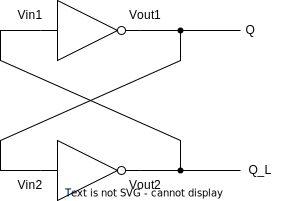
\includegraphics[width=0.35\textwidth]{figs/biestable.drawio.png}
	\caption{Biestable.}
	\label{fig:biestable}
\end{wrapfigure}

El biestable se llama así, porque el análisis digital muestra que tiene dos estados estables. Si Q es ALTO, entonces Q\_L es BAJO, lo cual refuerza el estado de Q. De esta manera tenemos dos estados estables, ALTO y BAJO. Lo mismo ocurre cuando Q es BAJO, ya que esto causa que Q\_L sea ALTO, lo que refuerza que Q sea BAJO. Al no disponer de ningún elemento de control o que nos permita cambiar el estado, al iniciar el biestable, este genera aleatoriamente el estado y se mantiene invariable para siempre.

\textcolor{red}{¿HABLAR DE METAESTABILIDAD AQUÍ?}

\subsection{Latches y biestables}
La diferencia entre latch y flip-flop es que mientras el latch refleja inmediatamente en la salida los cambios en la entrada, los flip-flops solo reflejan este cambio en los tics de reloj. A continuación se explican las diferentes variantes de latches y flip-flops.

\subsubsection{Latch S-R}

Los \hyperlink{sr_latch}{\emph{latch S-R}} son el circuito secuencial más simple que se puede construir y que tenga entradas de control. Se puede construir con dos puertas NOR de dos entradas (véase la Figura \ref{fig:latch-sr}). 

\begin{wrapfigure}{o}{0.4\textwidth}
    \centering
    \includegraphics[width=0.35\textwidth]{figs/latch-sr.drawio.png}
    \caption{Latch S-R.}
    \label{fig:latch-sr}
\end{wrapfigure}

La 'S' y la 'R' vienen del inglés \emph{set} y \emph{reset}, y son las señales de control del circuito. Las salidas se denominan 'Q' y 'QN' y no tienen por qué ser una el complemento de la otra, a pesar de que normalmente en la mayoría de las aplicaciones lo suele ser. Por ejemplo, como se observa en la Figura \ref{fig:wave-latch-sr2}, si S y R valen 1 en el mismo instante de tiempo, las salidas cambian ambas a 0. Además, si se niegan tanto S como R al mismo tiempo, el circuito entra en un estado de metaestabilidad, haciendo el siguiente estado de las salidas impredecible. No obstante, si las entradas se niegan en instantes diferentes, las salidas retienen el estado anterior. Esto otorga al circuito su capacidad de almacenamiento.

\begin{figure}[h]
    \centering
  
    \begin{subfigure}[b]{0.35\textwidth}
      \includegraphics[width=\textwidth]{figs/wavedrom-latch-sr.png}
      \caption{Operación normal de un latch S-R.}
      \label{fig:wave-latch-sr1}
    \end{subfigure}
    \hfill
    \begin{subfigure}[b]{0.55\textwidth}
      \includegraphics[width=\textwidth]{figs/wavedrom-latch-sr2.png}
      \caption{Operación anómala cuando 'S' y 'R' son afirmados a la vez.}
      \label{fig:wave-latch-sr2}
    \end{subfigure}
  
    \caption{Diagrama de ondas de un latch S-R}
    \label{fig:wave-latch-sr}
\end{figure}

\subsubsection{Latch $\overline{\text{S}}$-$\overline{\text{R}}$}
Los \emph{latch $\overline{S}$-$\overline{R}$} funcionan de manera similar a los anteriores, con la diferencia de que las entradas S y R son activas a nivel bajo. A diferencia de los latch S-R, estos pueden ser construidos a partir de puertas NAND. Debido a que las puertas NAND ofrecen ciertas ventajas sobre las NOR, en términos de velocidad y tamaño, estos latches suelen utilizarse más en cirtos contextos.

\subsubsection{Latch D}

\begin{wrapfigure}{o}{0.45\textwidth}
    \centering
    \includegraphics[width=0.4\textwidth]{figs/latch-d.drawio.png}
    \caption{Latch D.}
    \label{fig:latch-d}
\end{wrapfigure}

A pesar de que tanto el latch S-R como el $\overline{S}$-$\overline{R}$ pueden almacenar información, éstos se usan más en respuestas a ciertos cambios de condiciones del sistema que requieren reseteos. Para el almacenamiento de bits de información se utilizan otra clase de circuitos, que se verán a continuación. El primero de ellos es el \emph{latch D}.

Como se puede ver en la Figura \ref{fig:latch-d}, el latch D se construye sobre un latch $\overline{\text{S}}$-$\overline{\text{R}}$ al que se añaden dos puertas NAND con dos entradas: D, que es el dato que se quiere almacenar; y G, que es una señal de control que evita que se produzca la situación en la que tanto $\overline{\text{S}}$ como $\overline{\text{R}}$ sean afirmadas, dando lugar a metaestabilidad. De esta manera, 